\documentclass[11pt]{report}
%Libraries in alphabetical Order, Date added Tab Spaced after
\usepackage{amsmath}				%1-15-2015
\usepackage{caption}				%1-17-2015
\usepackage{floatflt}				%1-15-2015
\usepackage{graphics}				%1-15-2015
\usepackage{listings}             	%1-17-2015
\usepackage[pdftex]{graphicx}		%1-14-2015
\usepackage{subcaption}				%1-17-2015
\usepackage[xindy]{glossaries}		%1-14-2015
\usepackage{wrapfig,lipsum,booktabs}%2-8-2015
\usepackage[T1]{fontenc}
\usepackage{pdfpages}
\usepackage{multicol}

%		\begin{figure}[!ht]
% 		 \caption{X axis is number of nodes, Y axis is energy con%sumed. }
  %		 \centering
 %   	 \includegraphics[width=.9\textwidth]{Q3c.png}
%		\end{figure}


\begin{titlepage}
\title{
		\Huge{
				\textbf{ECE 6276
						\\DSP Hardware System Design
						\\Fall 2017}}
			\\[2cm]
		\LARGE{
			\textnormal{Lab 1}}
			\\[1cm]
			\date{\today}
		\large{
			\author{William Sutton}
		}}


\end{titlepage}

\usepackage{amsmath}
\begin{document}
\lstset{language=MATLAB}
\maketitle
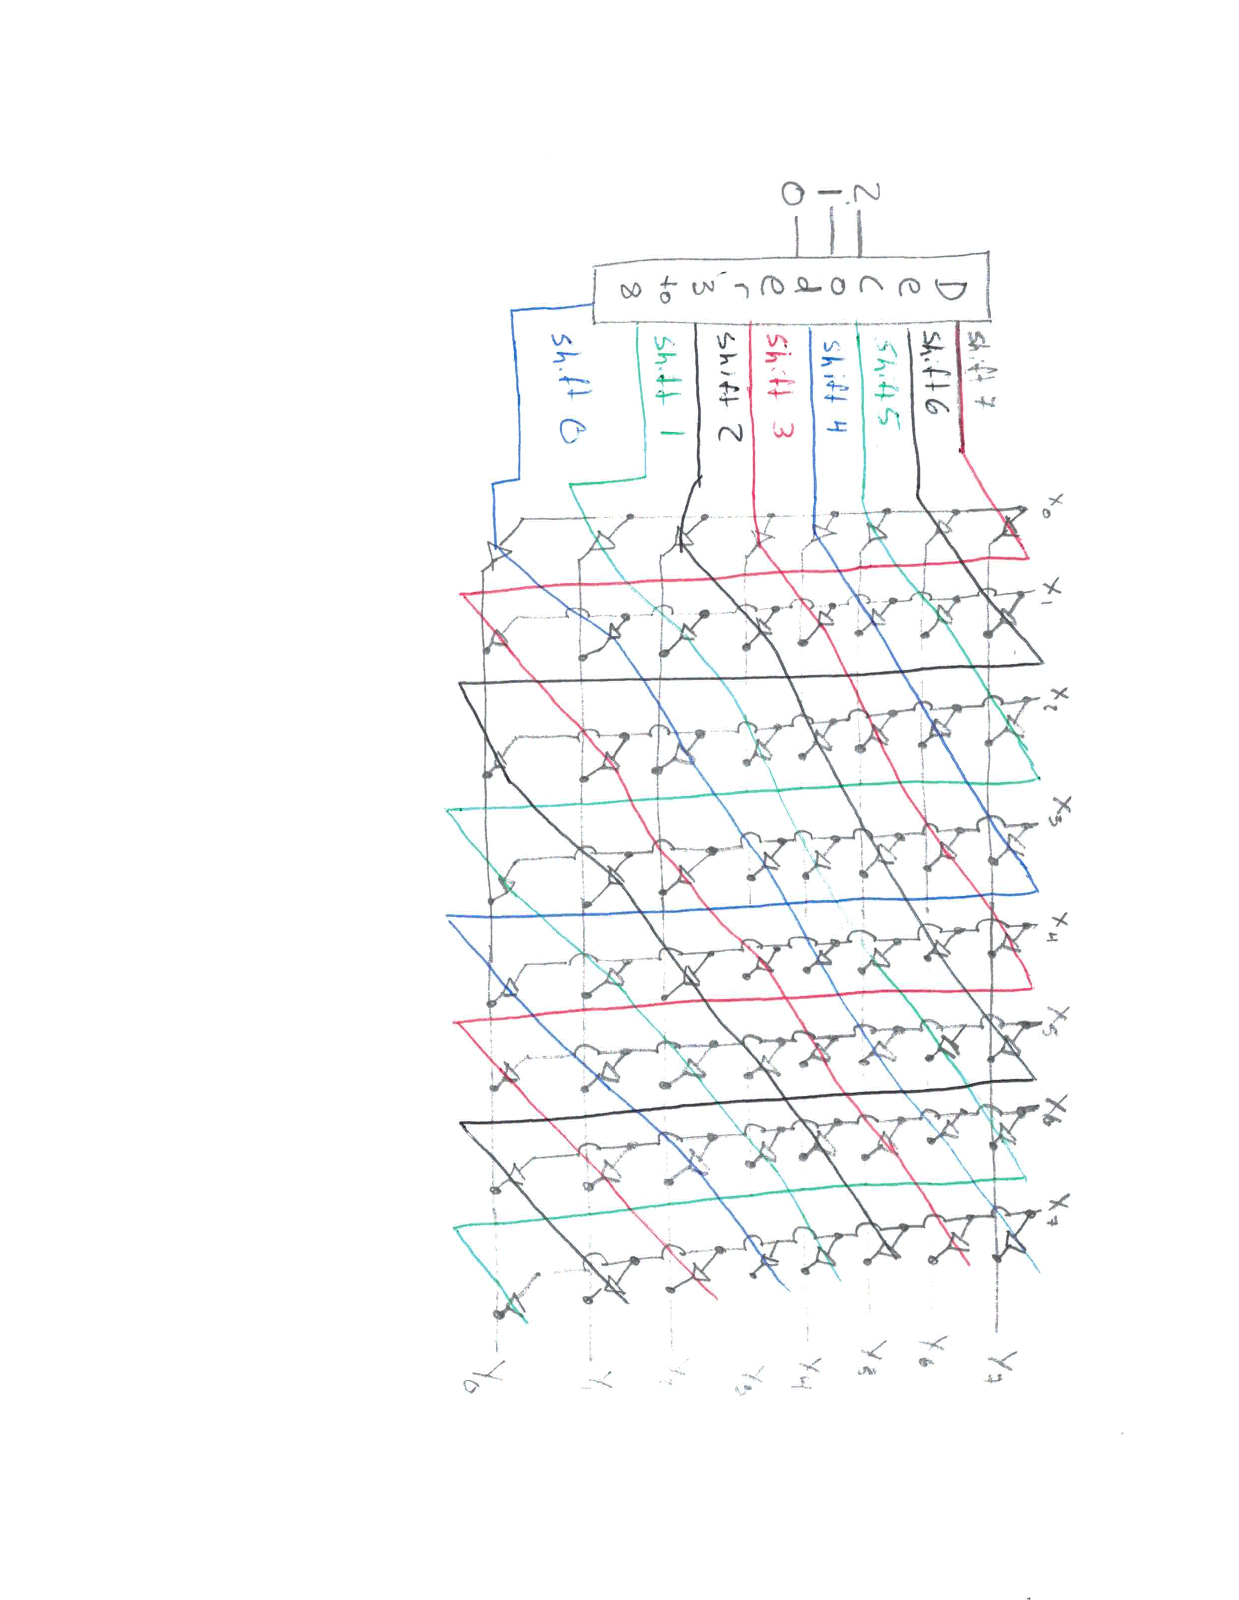
\includepdf[pages={1}]{BRN30055C8F6EB0_000502.pdf}
\newpage

		\begin{figure}[!ht]
 		 \caption{}
  		 \centering
    	 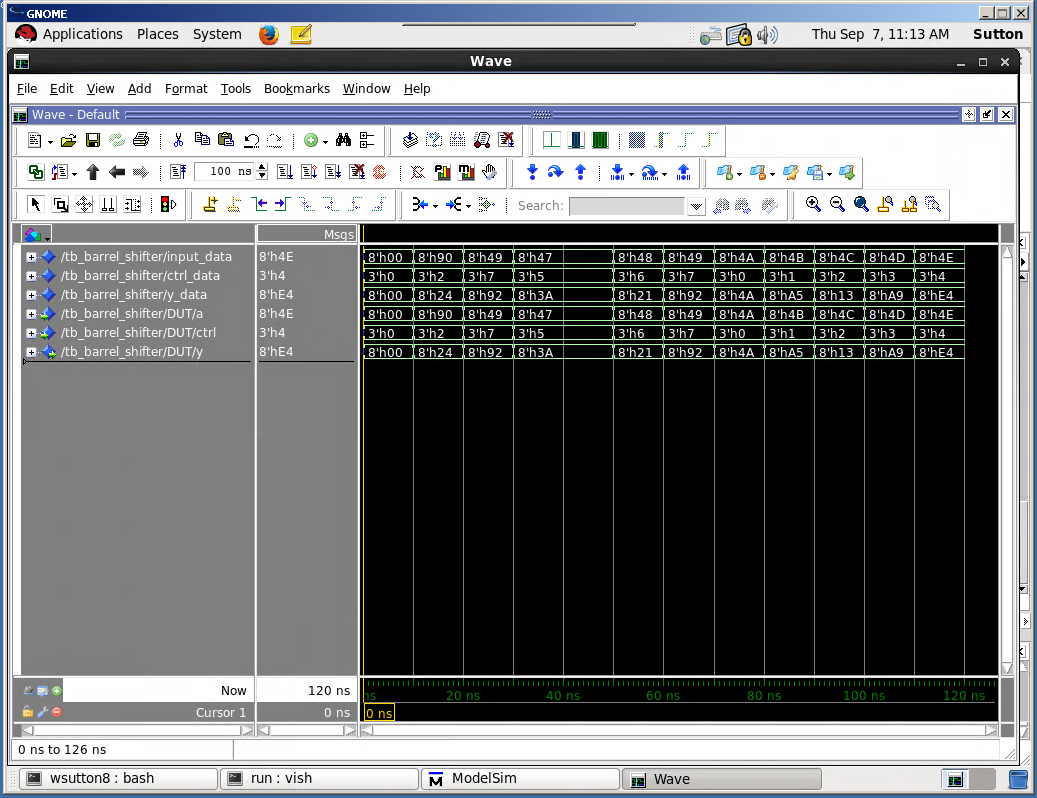
\includegraphics[width=1.2\textwidth]{Screenshot_2017-09-05_21-26-20.png}
		\end{figure}
		\newpage
		
\section*{Manual Verification}
Since the barrel shifter is essentially bit shifting with a carry function, we can simply move the data bits around. i.e.\\

0x90=0b10010000 $\rightarrow $by 0b011 = 0b00010010 = 0x12\\
0x49=0b01001001 $\rightarrow $by 0b110 = 0b00100101 = 0x25\\
0x47=0b01000111 $\rightarrow $by 0b001 = 0b10100011 = 0xA3\\
\section*{Answer to question in part iv}
No I don't think this is the best strategy used. This tests changing input data AND changing control information simultaneously. For a valid test, I would keep the data the same, while toggling the control pins. Then afterwards, I would toggle the data pins, while keeping the control pins the same. This would show full functionality.
\end{document}
